%!TEX root = ../thesis_phd.tex
%%%%%%%%%%%%%%%%%%%%%%%%%%%%%%%%%%%%%%%%%%%%%%%%%%%%%%%%%%%%%%%%%%%%%%%%%%%%%%%%
% experiment.tex: Chapter describing the experiment
%%%%%%%%%%%%%%%%%%%%%%%%%%%%%%%%%%%%%%%%%%%%%%%%%%%%%%%%%%%%%%%%%%%%%%%%%%%%%%%%
\chapter{\nova}
\label{nova_chapter}
Neutrinos at the Main Injector (\numi) is a high-intensity neutrino source located at Fermilab.  The \numi Off-axis \nue Appearance (\nova) experiment will employ this source in one of the latest efforts in the class of long baseline neutrino experiments.  Long baseline neutrino experiments aim to observe neutrino oscillations in a detector placed at some long distance -- known as the baseline -- from a neutrino source.  \nova employs two detectors for observation of neutrinos, one near the source and another 810 km away in Ash River, Minnesota.  The Near Detector (ND) is used to observe the initial  \numi flux at a distance where oscillations are negligible; the Far Detector (FD) observes the \numi flux subject to neutrino oscillations.  \numi will be discussed in section~\ref{sec:numi}, and the \nova detectors in \ref{sec:detectors}.  The detectors are comprised of long cells which are arranged horizontally

\nova aims to provide precision measurements of \thetaoth and \thetatth though sensitivity to the probabilities $P(\nu_\mu \rightarrow \nu_\mu)$ and $P(\nu_\mu \rightarrow \nu_e)$.  Preliminary measurements of nonzero measurement of \thetaoth are consistent with measurements from Daya Bay, RENO and T2K \cite{nova2016nue}.  It is also hoped that \nova will  hone the measurement of \thetatth to determine whether it is greater or less than $45^\circ$.  This thesis aims to further techniques which will aid in both of these efforts, although we focus on the applicaiton to muon neutrino identification for meaurement of \thetatth.

Unique to accelerator neutrino experiments like \nova is the ability to produce either neutrinos or antineutrinos.  The matter effect, as described in section~\ref{matOsc}, predicts a difference between the appearance probabilities for neutrinos and antineutrinos.   By comparing the respective appearance probabilities, it could be possible to determine whether the mass hierarchy is normal or inverted.  The difference between neutrinos and antineutrinos could also be used to measure the CP violating phase, $\delta$.


\section{\numi and  Off-axis Alignment }\label{sec:numi}

In a process similar to the Brookhaven experiment that discovered the muon neutrino, the \numi beam is generated by protons accelerated to 120 GeV by the Main Injector at Fermilab.  A schematic of the \numi configuration can be seen in Figure~\ref{numi}.

Protons from the Main Injector are directed into a graphite target producing a shower of hadrons including pions and kaons.  The hadron showers are focused into a beam by the magnetic field produced in ``focusing horns,'' which are tuned to select charged pions by steering them forward while steering other particles out of the beam.  Downstream of the focusing horns, particles are free to decay in flight inside a 675 m decay pipe.  Muon neutrinos are then produced when charged pions decay as shown in equation \eqref{pions}.  Alternatively, anti-pions can be focused by switching the direction of the electric current in the focusing horns, thus \numi can serve as either a neutrino or antineutrino beam.  A small component of kaons and other heavier mesons which pass through the focusing horns.  Heavy mesons can decay to electrons and \nue at higher rates, which introduces electron neutrino background in the predominantly \numu beam.  Charged particles such as muons and electrons produced in the decay pipe are absorbed in rock upstream of the \nova Near Detector, eliminating them as background.  The \numi facility can achieve an intensity of 700 kW by delivering bunches of $4.9 \times 10^{13}$ protons to the target every 1.3 seconds \cite{tdr}.

\begin{figure}[t]
  \begin{center}
    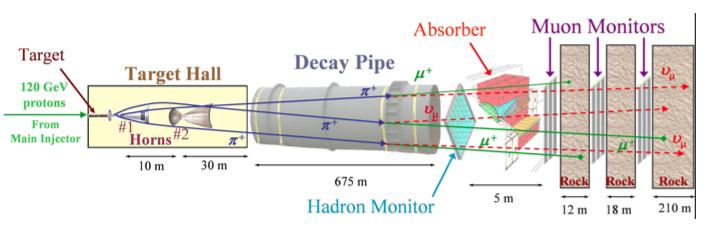
\includegraphics[width=\textwidth]{figures/figures/numi.png}
  \end{center}
  \caption[A schematic of the \numi neutrino source.]{A schematic of the \numi neutrino source.  Courtesy of Robert Zwaska \cite{zwaska2005thesis}.}
  \label{numi}
\end{figure}

Rather than being placed directly in the \numi beam line, the \nova detectors are placed 14.6 milliradians off of the beam axis.  As displayed in Figure~\ref{EnuEpi}, the neutrinos produced on-axis demonstrate a strong dependence on the parent pion energy, as opposed to the weak energy dependence of those produced slightly off-axis.  Since the pions produced at the target have a spread of energies, this weak dependence helps to narrow the neutrino energy spectrum, as seen in Figure~\ref{fluxEnu}.  The neutrino energy spectrum at 14.6 milliradians is characterized by a sharp peak near 2 GeV.  \nova's FD has been placed with baseline of 810 km to take advantage of an oscillation minimum between 1 and 2 GeV.  Further, the narrowness of the peak reduces the fraction of the spectrum above 2 GeV.  Neutral current neutrino interactions produce only a small amount of visible energy since a large fraction is carried away by the outgoing neutrino.  High energy neutral-current background events can be misidentified as charged-current signal events, so the narrow energy peak helps reduce this background.
\begin{figure}[t]
\centering
\begin{subfigure}[c]{0.8\textwidth}
                \centering
                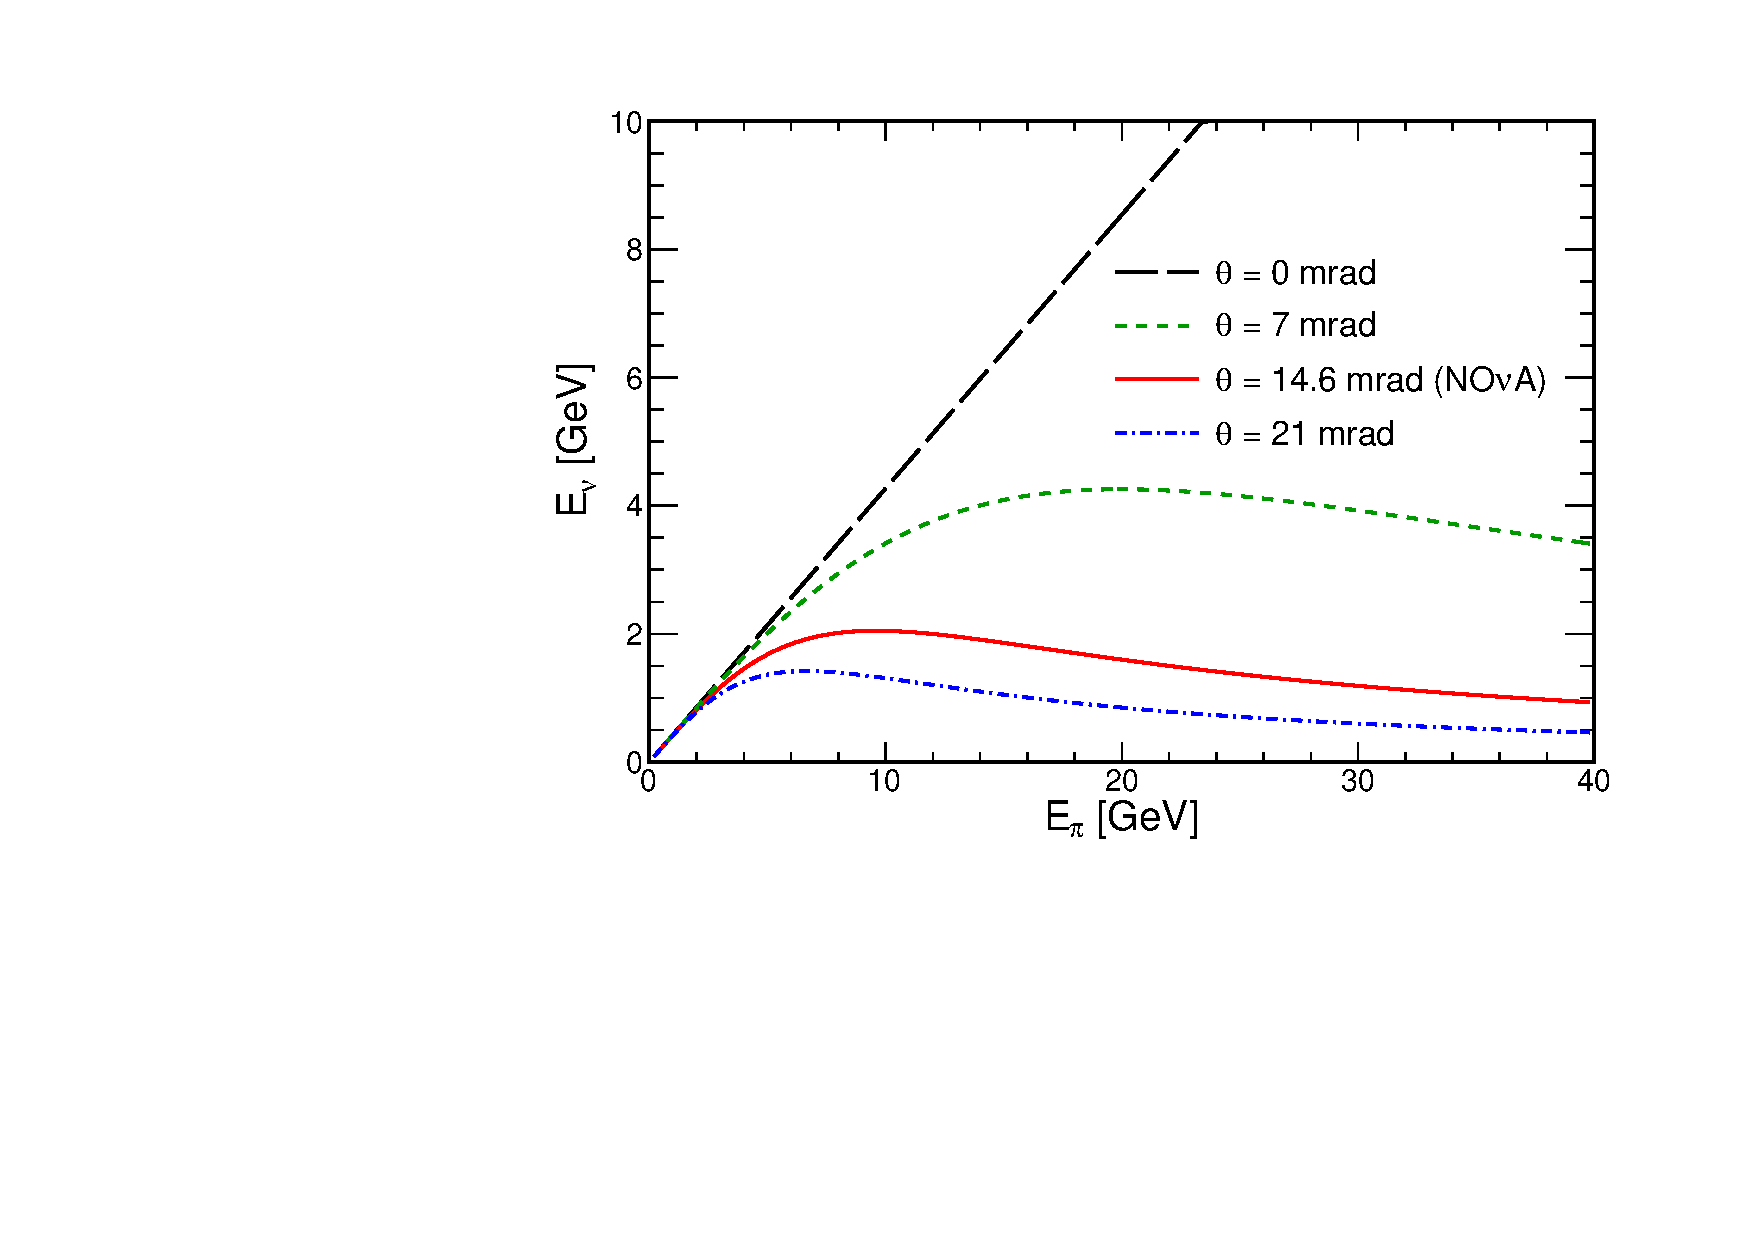
\includegraphics[width=\textwidth]{figures/plots/nova/EnuVSEpi_NOvA-0-7-21.pdf}
                \caption{Neutrino energy vs. pion energy at various angles relative to the beam axis.}
                 \label{EnuEpi}
        \end{subfigure}


\begin{subfigure}[c]{0.8\textwidth}
                \centering
                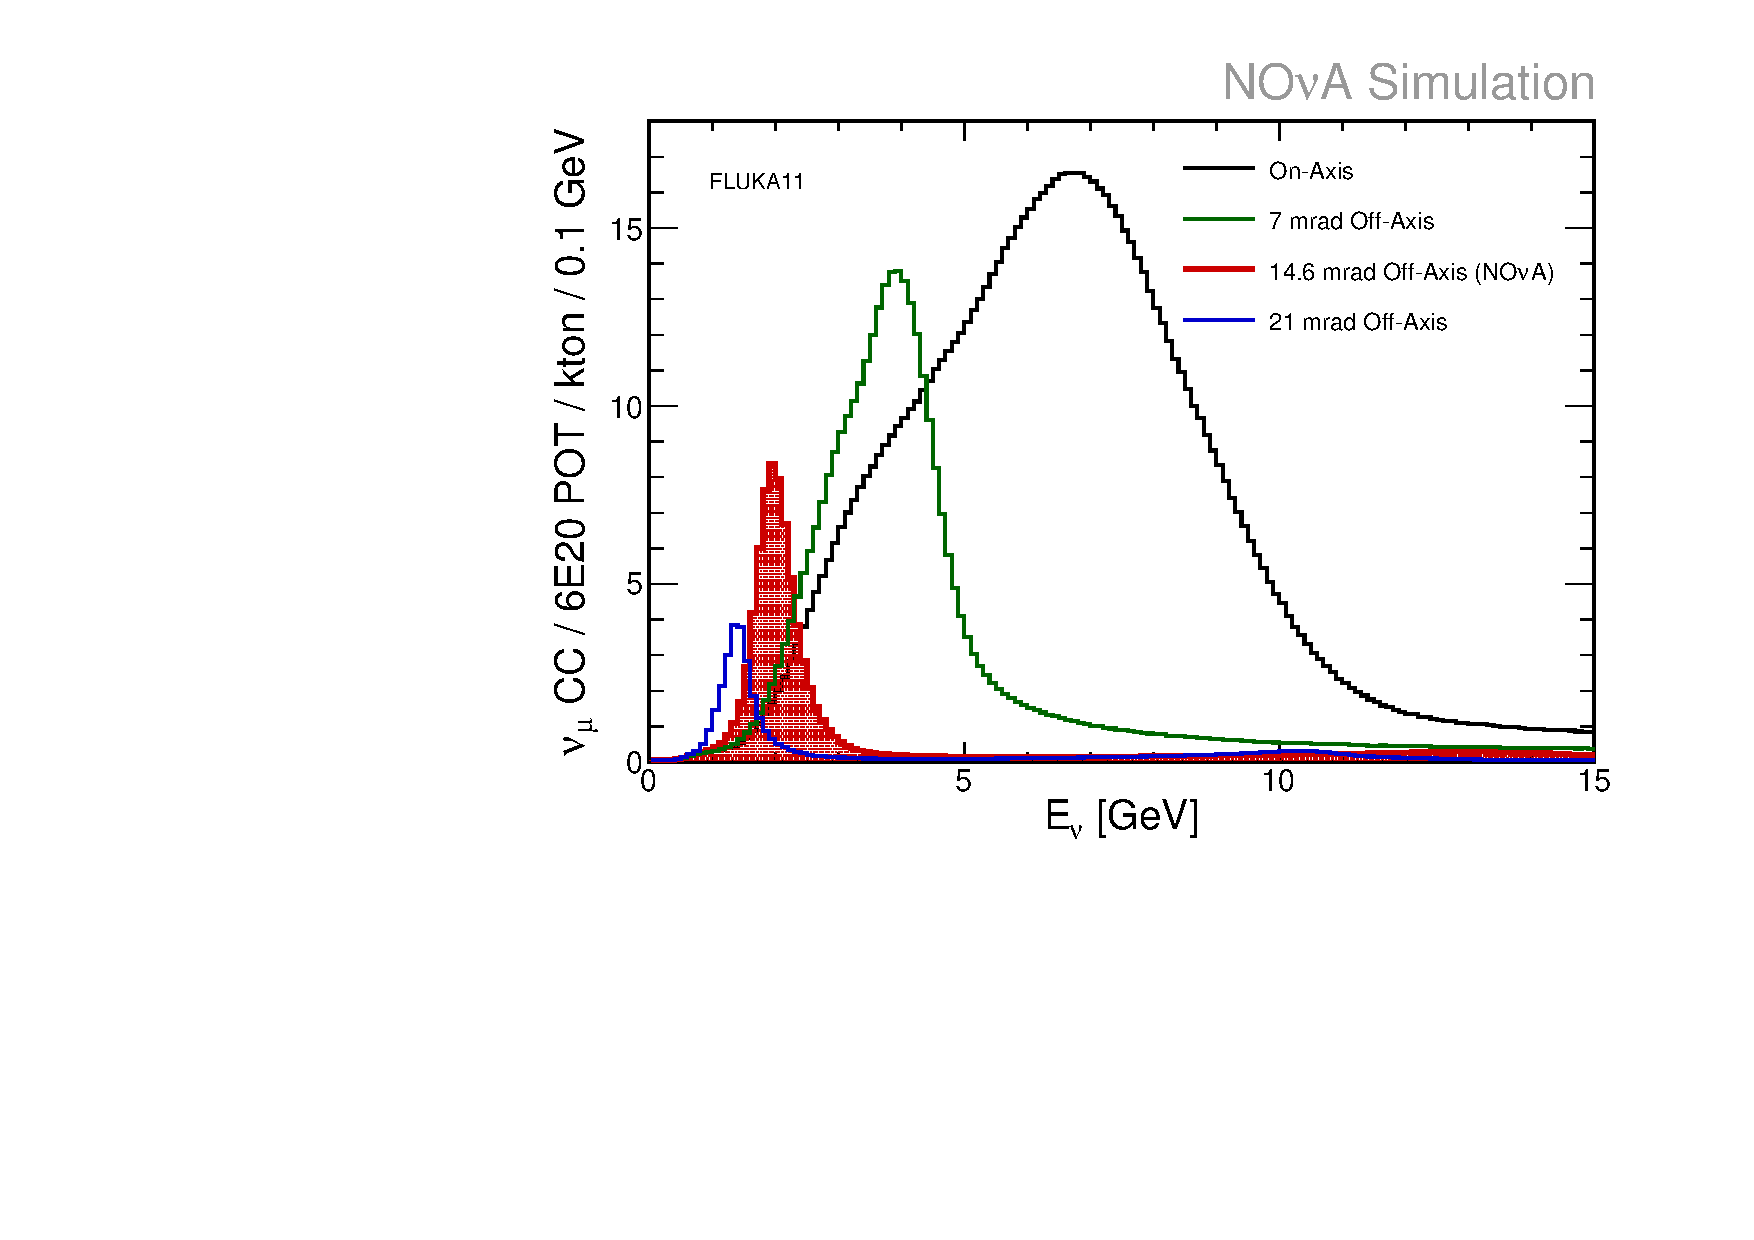
\includegraphics[width=\textwidth]{figures/plots/nova/spectrum_FD_NOvA-0-7-21.pdf}
                \caption{Expected \numu event counts vs. neutrino energy at various angles relative to the beam axis}
                \label{fluxEnu}

        \end{subfigure}
        \caption{Effects of off-axis design.}
\end{figure}

\section{\nova Detectors}
\label{sec:detectors}

\begin{figure}[t]
\begin{subfigure}[t]{0.25\textwidth}
                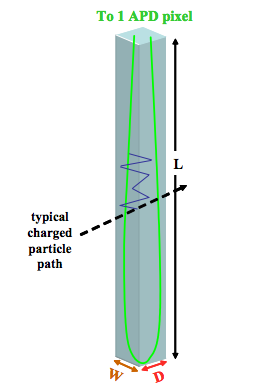
\includegraphics[height=0.35\textheight]{figures/figures/cell.png}
               \caption{A NO$\nu A$ cell.}
                 \label{cell}
        \end{subfigure}
        ~
\begin{subfigure}[t]{0.75\textwidth}
                \centering
                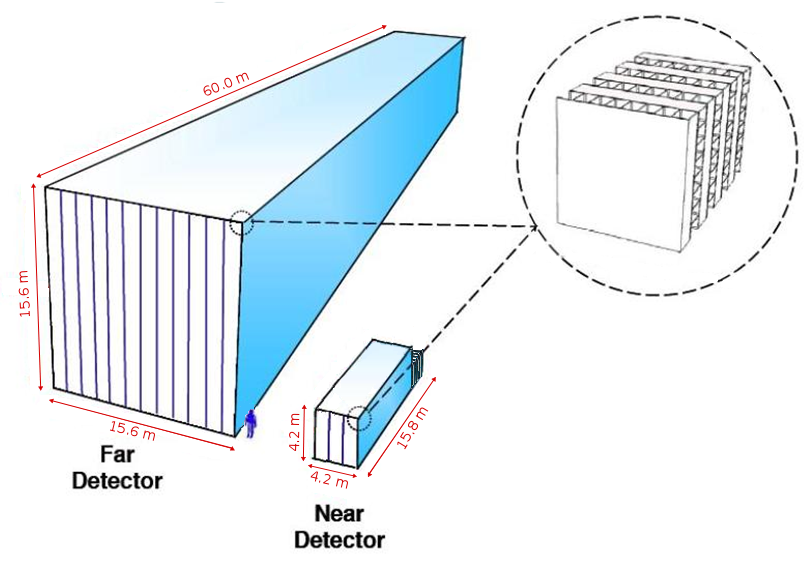
\includegraphics[height=0.35\textheight]{figures/figures/detectors.png}
               \caption{Scale and topology of the \nova detectors.}
                \label{detector}

        \end{subfigure}
        \caption{Drawings of the \nova detectors}
\end{figure}

 The \nova detectors are designed to allow fine-grained reconstruction of electromagnetic and hadronic showers.
 Such a detailed view can allow identification of \numu and \nue CC
 interactions, and help to tell them apart from NC interactions.  To achieve this goal, the detector topology is a repeated structure of unit cells which are much smaller than the electromagnetic and strong interaction lengths of the composite materials.  Charged particles produce light as they traverse the cells, which enables detection.  Cells are long, but arranged in alternating horizontal and vertical planes to provide measurements of Cartesian coordinates.
 Example event topologies can be seen in Figure \ref{eventtopnue}.
 The detectors are designed to be functionally identical to each other; they are built with the same materials and geometry to constrain systematic uncertainties due to variation in detector efficiency.

\begin{figure}[t]
\begin{center}
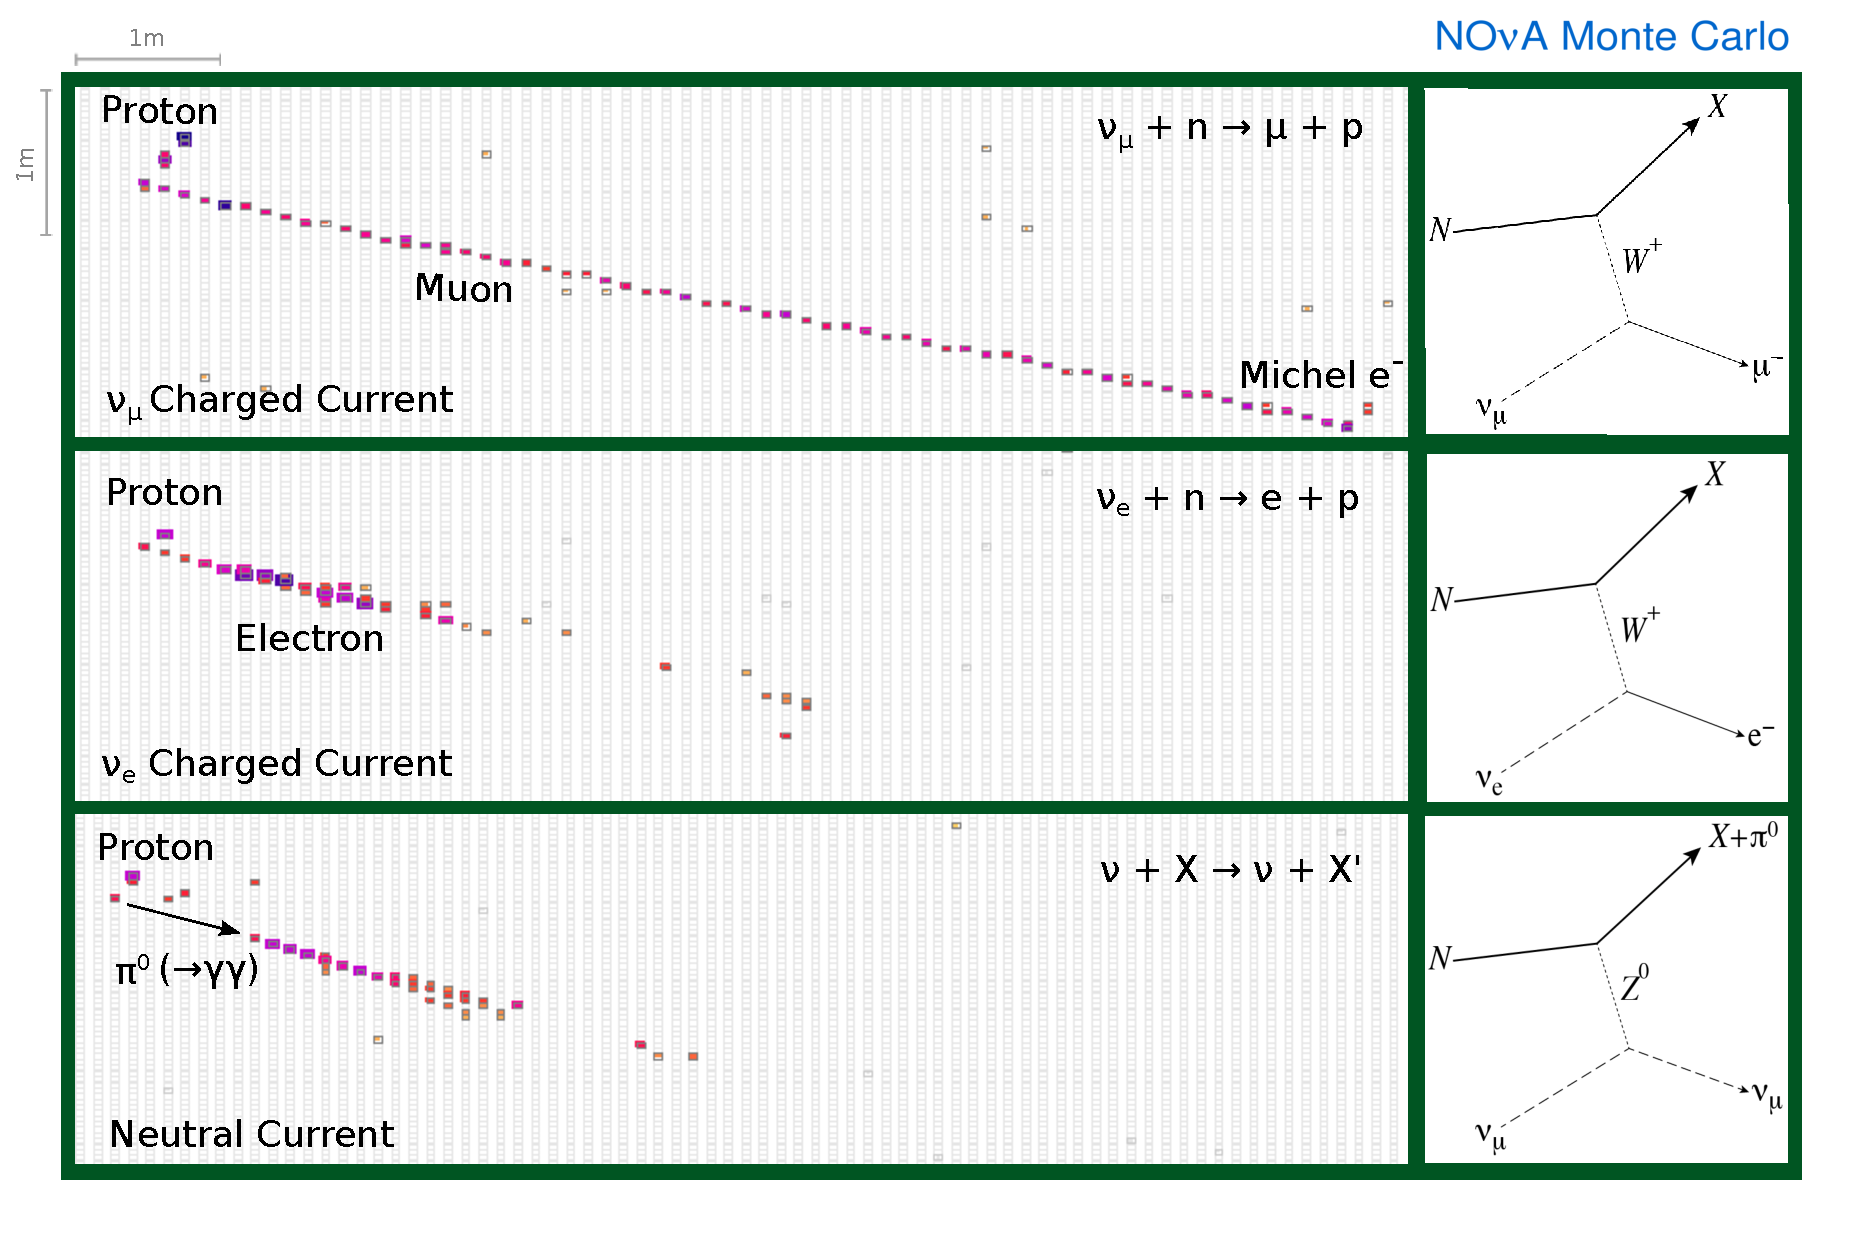
\includegraphics[width=\textwidth]{figures/figures/event_topology_nue.pdf}
\end{center}
\caption{Event topologies in \nova}{Shown are three example event topologies in
\nova.  The top pane shows a \numu CC interaction with a long muon track and
visible activity from a proton.  An electron shower from a \nue CC interaction
is visible in the middle pane.  The third pane shows a NC interaction
with a neutral pion decaying to two photons, which forms the dominant
background in \nova's \nue appearance search.The electromagnetic
radiation length in \nova is relatively long compared to the size of a cell,
which aids in distingusing such events.}
\label{eventtopnue}
\end{figure}


\subsection{Cell Structure}
\label{cell_section}
 The rigid structure of the cells is comprised of tubular \textit{cells} extruded from poly-vinyl chloride (PVC) resin.  Each cell is approximately 4 cm wide and 6 cm deep; FD cells are nearly 15 m long, while ND cells are about 4 m long.  Cells are arrayed into planes, the detector is assembled from arrayed planes, with adjacent planes alternating between horizontal and vertical rotations.  Configured in this way, cells allow Cartesian coordinates to be inferred; vertical cells provide a measurement of the $x$-coordinate, horizontal cells they $y$-coordinate, and planes the $z$-coordinate.  A visualization of the detector topology can be seen in Figure \ref{detector}.

 Cells are aligned side-by-side (along the 6 cm side) into units of 32 cells referred to as a modules.  Planes are thus a collection of adjacent modules which are glued face-to-face to produce detector \textit{blocks}.  In the FD, planes are 12 modules wide, blocks contain 32 planes, and the complete detector is 28 blocks.  The ND has three blocks of 24 planes, each of which is 3 modules wide.  Additionally, the ND is augmented with an extra downstream block known as the \textit{muon catcher}.  As its name suggests, this block is designed to range out muons, which can traverse a range of several meters from the \numu CC interactions seen  in \nova.  Interleaved between each pair of horizontal and vertical modules in the muon catcher is a 10 cm plane of steel.  Steel absorbs extra energy from the muons so that they will range out within the detector, thus allowing their total energy to be estimated based on their range.  The muon catcher is comprised of 22 active planes interleaved with 10 steel planes.  Muon catcher planes are three modules wide for vertical planes, but only two modules tall for horizontal planes.

\begin{figure}[t]
\begin{center}
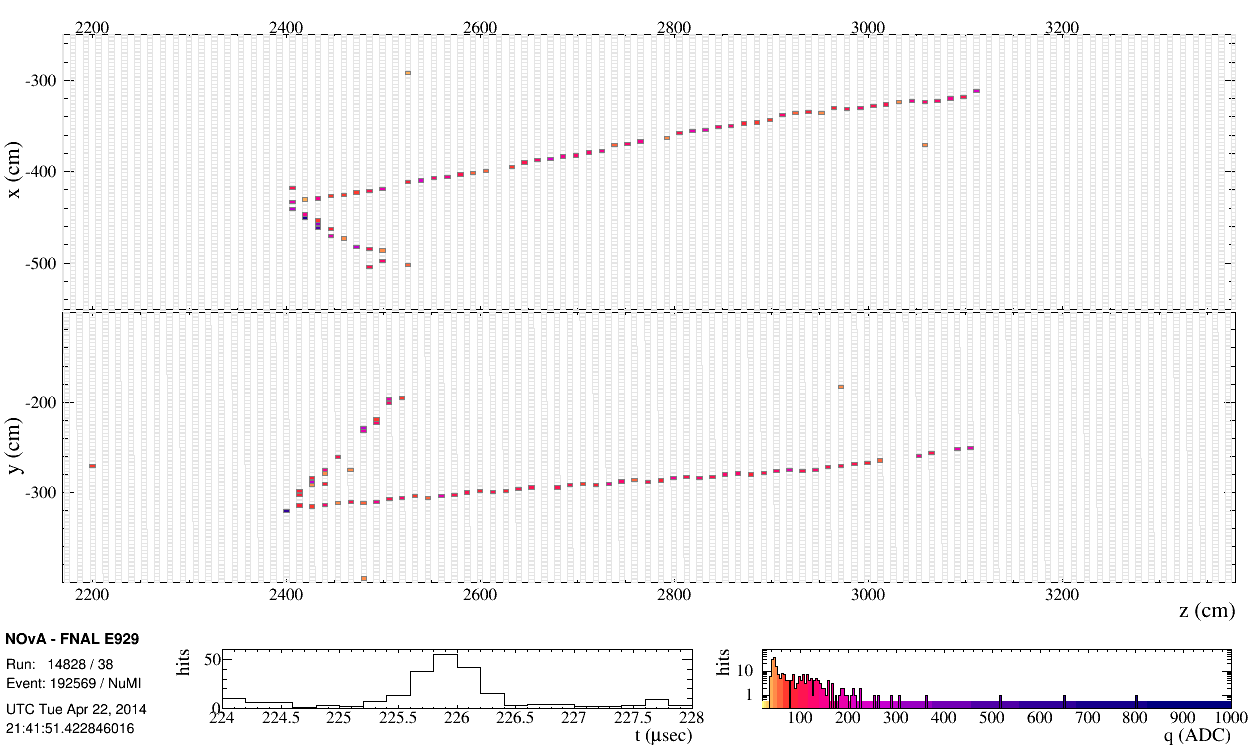
\includegraphics[width=\textwidth]{figures/evd/evd_numu_cand.png}
\end{center}
\caption{An example \nova event display.  The top projection is an $x$ vs. $z$ view, the bottom is $y$ vs. $z$.  This is a candidate \numu charged-current event from in the Far Detector.}
\label{eventDisplay}
\end{figure}

\subsection{Light Collection}

Each cell is filled with scintillator-doped mineral oil to produce light in the presence of swiftly moving charged particles.  The mixture is roughly 95\% mineral oil by mass, blended with a primary scintillant which produces UV light and two wavelength shifting components \cite{mufson2015liquid}.  A strand of wavelength-shifting fiber runs up and down the length of each cell with both ends of fiber emerging at one end of the cell, visualized in figure~\ref{cell}.  The fiber serves the purpose of capturing and transmitting the scintillation light in two steps; first by lengthening its wavelength through molecular absorption and reemission, and then trapping it within the fiber by total internal reflection.

At the end of the cells, photons trapped in the WLS fiber are converted to photo-electrons on an avalanche photodiode (APD) to produce an electrical signal.  The signal One APD board contains 32 pixels to read out each cell of module separately.  APD signals are read out by four electronic components built into a front end board (FEB) designed specifically for \nova.  An application specific integrated circuit (ASIC) shapes the pulses.  The ASIC is CR-RC circuit which amplifies and widens the signals in time to better distinguish physics signals from noise.   Shaped pulses are passed to an analog-to-digital converter (ADC) which samples at 64 MHz time-to-digital (TDC) clock-ticks.  The sampling of the 32 pixels is multiplexed, eight-fold in the FD and two-fold in the ND.  Zero suppression of the ADC samples is performed by a field programmable gate array (FPGA) which employs a dual correlated sampling (DCS) technique to trigger a hit to be passed to the data acquisition (DAQ) system.  Under the DCS scheme, each ADC sample the third latest sample.  If the difference between those two samples is greater than a fixed threshold, a hit is passed along to be recorded by the DAQ.

\subsection{Data Acquisition}

The \nova data concentrator module (DCM) is responsible for collecting data from up to 64 APD/FEB pairs.   A DCM is a device mounted on the detector with an embedded CPU running Linux and custom \nova DAQ software.  Input and output is transmitted using a standard CAT5e link network link.  Output from a DCM is transmitted to a buffer farm over 200 compute nodes.  These nodes are arranged to store data in a circular ring buffer, or in other words, when new data arrives, the oldest data is overwritten.  The buffer farm is capable of storing FD data for upwards of several minutes, during which time any subset of the buffered data can be written to disk and stored permanently.  Trigger decisions are issued through the custom \nova global trigger software, which can receive external triggers as well as data-driven triggers based analysis of data stored in the buffer farm.  This thesis primarily external triggers.  Neutrino data is recorded in the ND and FD by the so-called \numi trigger, which records 550 $\mu$s of data centered around the 10 $\mu$s \numi beam spill.  FD Cosmic ray data -- used for calibration and background estimation -- is recorded using a 10 Hz minimum bias trigger, commonly referred to as the cosmic trigger.   Cosmic events in the ND are a commodity since the detector is underground; a minimum bias trigger at any sampling rate simply does not record enough activity.  In place such a trigger, an simple activity based data-driven trigger is used to collect cosmic ray data in the ND.  This trigger reads out data whenever certain number of hits are recorded above a certain threshold.

Data is written to computer hard disks at the respective ND and FD sites.  Each site is capable of storing many days worth of data.  Ultimately, the data is transfered to Fermilab for permanent storage, where it is archived on tape and made available for offline reconstruction and physics analysis.


\subsection{Exposure}


In order to scale distributions of selected events, careful tracking
of exposure is necessary.
The important measures of exposure for \nova are livetime,
protons-on-target (POT), and detector mass.
Livetime is used for scaling constant processes
like cosmic rays and electronic noise.
Exposure to neutrinos, however, is prortional to the number decayed pions
in the \numi beam.
The number of pions depends on the number of protons delivered to the target,
which is tracked spill-by-spill and recorded in a database.
\nova detectors can also be operated in configurations which leave blocks
out of the readout, so careful tracking of active detector mass is also
necessary for accurate normalization.


%%%%%%%%%%%%%%%%%%%%%%%%%%%%%%%%%%%%%%%%%%%%%%%%%%%%%%%%%%%%%%%%%%%%%%%%%%%%%%%%
